\documentclass[11pt]{ctexart}
% \documentclass{article}
\textheight 23.5cm \textwidth 15.8cm
%\leftskip -1cm
\topmargin -1.5cm \oddsidemargin 0.3cm \evensidemargin -0.3cm

\usepackage{verbatim}
\usepackage{fancyhdr}
\usepackage{graphicx}
\usepackage{amssymb}
\usepackage{amsmath}
\usepackage{booktabs}
\usepackage{subcaption}
\usepackage{listings}
\usepackage{color}
\usepackage{geometry}


\definecolor{mygreen}{rgb}{0,0.6,0}
\definecolor{mygray}{rgb}{0.5,0.5,0.5}
\definecolor{mymauve}{rgb}{0.58,0,0.82}

\lstset{
  language=Matlab,                % 设定语言为MATLAB
  frame=single,                   % 外围框架
  basicstyle=\footnotesize\ttfamily,   % 基本代码风格
  keywordstyle=\color{blue},      % 关键词风格
  commentstyle=\color{mygreen},   % 注释风格
  stringstyle=\color{mymauve},    % 字符串风格
  numbers=left,                   % 行号位置
  numberstyle=\tiny\color{mygray}, % 行号风格
  stepnumber=1,                   % 行号步长
  numbersep=5pt,                  % 行号与代码间隔
  backgroundcolor=\color{white},  % 代码背景色
  showspaces=false,               % 不显示空格
  showstringspaces=false,         % 不显示字符串中的空格
  showtabs=false,                 % 不显示制表符
  tabsize=4,                      % 制表符宽度
  captionpos=b,                   % 标题位置
  breaklines=true,                % 自动换行
  breakatwhitespace=false,        % 仅在空格处换行
  escapeinside={\%*}{*)},         % 可以添加LaTeX内容
}


\ctexset {
     section/format    += \sffamily\raggedright,
     subsection/format += \fbox,
}

\title{FEM Report4}
\author{SA24229016 王润泽}

\begin{document}
\maketitle

\section{Introduction}
编写程序求解 $ \Omega=[0,1]\times [0,1] $定义域范围的 Dirichlet边值问题:
\begin{equation}
     \begin{aligned}
         -\nabla^2 u &= f \quad \text{in } \Omega, \\
         u &= 0 \quad \text{on } \partial \Omega.
     \end{aligned}
\end{equation}
有限元空间选取为分段连续线性多项式空间 $ V_h $且准确解为 $ u(x,y) = (x-1)\sin(x)(y-1)\sin(y) $。

\section{Algorithm}

\subsection{Variational Formulation}
首先将 Dirichlet边值问题转化为如下变分问题:

定义双线性形式:

$$ a(u,v) = \int_{\Omega} \nabla u \cdot \nabla v \, dx dy $$ 

线性形式 
$$ L(v) = \int_{\Omega} f v \, dx dy .$$

那么问题(1)的变分问题为:求 $ u \in V = \{ v \in H^1(\Omega) : v|_{\partial \Omega} = 0 \} $ ,使得对于所有 $ v \in V $ ,有:
\begin{equation}
     a(u,v) = L(v).
\end{equation}

\subsection{Finite Element Space}

对于二维有限元问题,我们采用三角剖分的方法,将二维区域剖分为三角形网格集合 $ \mathcal{T}_h=\{k_i\} $ ,每个三角形 上定义一个局部的有限元空间。如图所示,三角网格面元单元数为 $ 2N^2 $,内部顶点数为 $ (N-1)^2 $,边界顶点数为 $ 4N$。
\begin{figure}[htbp]
      \centering
      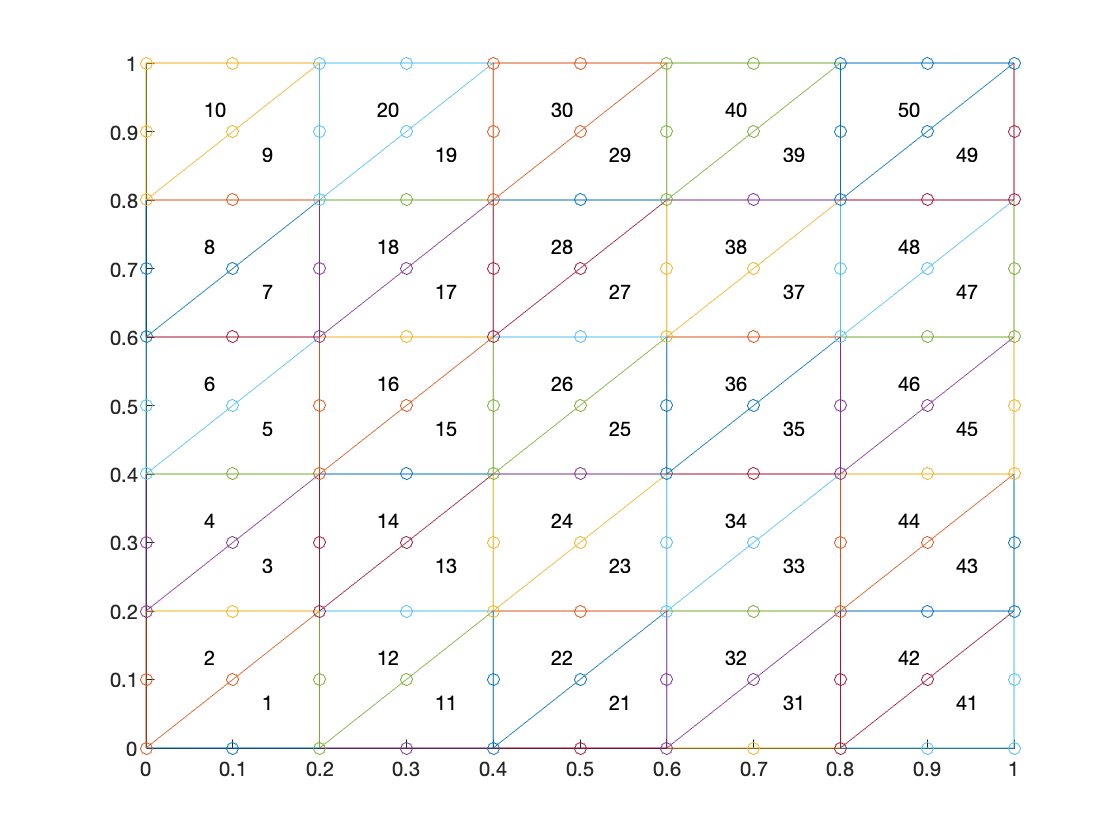
\includegraphics[width=0.5\textwidth]{triangulation.png}
      \caption{Triangulation}
      \label{fig:triangulation}
\end{figure}


对于每个三角形 $ k\in \mathcal{T}_h $ ,由其三个顶点定义 $ P_1,P_2,P_3 $ ,我们选取一个分段线性多项式空间作为局部的基函数 $ u(x,y) $:
\begin{equation}
      u(x,y) = ax+by+c,
\end{equation}
在三角形顶点处满足 $ u(x_i,y_i) = u_i $ ,其中 $ (x_i,y_i) $ 为三角形顶点坐标,$ u_i $ 为顶点处的值,$ i=1,2,3 $,$ u_i $ 即为待求解的值。将 $ u(x,y) $ 转换成重心坐标的形式:
\begin{equation}
    \begin{aligned}
      &u(x,y) = u_1 N_1(x,y) + u_2 N_2(x,y) + u_3 N_3(x,y)=\mathbf{N}^T \mathbf{u}\\
      &N_i(x,y) = \frac{1}{2\Delta_k} (a_i x + b_i y + c_i)\\
      &a_i = y_j-y_m, \quad b_i = x_m-x_j, \quad c_i = x_j y_m - x_m y_j
    \end{aligned}
\end{equation}
$ N_i(x,y) $ 为重心坐标函数, $ \Delta_k $ 为三角形面积, $ i,j,m $ 为三角形顶点编号,下标符合轮换对称性。注意:每个三角形的重心坐标 $ \mathbf{N}_k $ 都是依赖于三角形的顶点坐标的。

此时,我们可以得到局部基函数的表达式,进而得到整个区域的基函数,定义有限元空间 $ V_h $ :
\begin{equation}
      V_h = \{ v_h \in C(\Omega) : v_h|_k \in P_1(k), \forall k \in \mathcal{T}_h, v_h|_{\partial \Omega} = 0 \}.
\end{equation}

那么变分问题(2)转化为:求 $ u_h \in V_h $ ,使得对于所有 $ v_h \in V_h $ ,有:
\begin{equation}
     a(u_h,v_h) = L(v_h).
\end{equation}

\subsection{Numerical Integration}
设 $ u_h $ 为:
\begin{equation}
      u_h = \sum_{k\in \mathcal{T}_h} \mathbf{N}_k^T\mathbf{u}_k
\end{equation}
其中,$ u^k $ 为待求解的系数,对于共享顶点 $ P_i $ 的两个三角形 $ k_1,k_2 $ ,有 $ u_i^{k_1} = u_i^{k_2} $。

对三角形 $ k $ 区域内的基函数 $ u_k $ 求偏导数,得到:
\begin{equation}
  \begin{aligned}
    \nabla u_k(x,y) &= \nabla\mathbf{N}_k^T(x,y) \mathbf{u}^k\\
    &=\frac{1}{2\Delta_k}\begin{bmatrix}
      a_1^k & a_2^k & a_3^k\\
      b_1^k & b_2^k & b_3^k
    \end{bmatrix}\mathbf{u}_k\\
    &=\mathbf{B}_k\mathbf{u}_k
  \end{aligned}
\end{equation}

由此,双线性泛函 $ a(u_h,v_h) $ 可以写成:
\begin{equation}
  \begin{aligned}
    a(u_h,v_h) &= \sum_{k\in \mathcal{T}_h} \int_{k} \nabla \mathbf{u}_k^T \nabla \mathbf{v}_k \, dx dy\\
    &= \sum_{k\in \mathcal{T}_h} \int_{k} \mathbf{u}_k^T \mathbf{B}_k^T \mathbf{B}_k \mathbf{v}_k \, dx dy\\
    &= \sum_{k\in \mathcal{T}_h} \mathbf{u}_k^T \mathbf{A}_k \mathbf{v}_k
  \end{aligned}
\end{equation}
其中,$ \mathbf{A}_k = \int_{k} \mathbf{B}_k^T \mathbf{B}_k \, dx dy $ 为局部刚度矩阵。

同理,线性泛函 $ F(v_h) $ 可以写成:
\begin{equation}
  \begin{aligned}
    F(v_h) &= \sum_{k\in \mathcal{T}_h} \int_{k} f \mathbf{v}_k \, dx dy\\
    &= \sum_{k\in \mathcal{T}_h} \int_{k} f \mathbf{N}_k \mathbf{v}_k \, dx dy\\
    &= \sum_{k\in \mathcal{T}_h} \mathbf{b}_k^T \mathbf{v}_k
  \end{aligned}
\end{equation}
其中,$ \mathbf{b}_k = \int_{k} f(x,y) \mathbf{N}_k(x,y) \, dx dy $ 为局部载荷向量。

因此只需求解线性方程组:
\begin{equation}
  \begin{aligned}
    \mathbf{u}^T \mathbf{A} \mathbf{v} &= \mathbf{b}^T \mathbf{v}, \quad \forall \mathbf{v} \in V_h\\
    \leftrightarrow \quad \mathbf{A} \mathbf{u} &= \mathbf{b}
  \end{aligned}
\end{equation}
其中,$ \mathbf{A} = \sum_{k\in \mathcal{T}_h} \mathbf{A}_k $ 为全局刚度矩阵,为对称正定矩阵,$ \mathbf{b} = \sum_{k\in \mathcal{T}_h} \mathbf{b}_k $ 为全局载荷向量。

\subsection{Numerical Results}
我们采取如图1所示的等分剖分,每个三角形的直角边长为 $ h=1/N$ ,共有 $ 2N^2 $ 个三角形,$ (N+1)^2 $ 个顶点。

这样每个三角形的面积为 $ \Delta_k = h^2/2 $ ,如果选择顶点索引时,始终让直角边出现在三角形的第二个标号上,且采用逆时针顺序规划索引,那么局部刚度矩阵为:
\begin{equation}
  \mathbf{A}_k = \begin{bmatrix}
    1/2 & -1/2 & 0\\
    -1/2 & 1 & -1/2\\
    0 & -1/2 & 1/2
  \end{bmatrix}
\end{equation}

在构造全局刚度矩阵时,只需将局部刚度矩阵 $ \mathbf{A}_k $ 按照顶点索引的位置加到全局刚度矩阵 $ \mathbf{A} $ 的对应位置上即可。比如,对于三角形 $ k $ 的局部刚度矩阵的元素 $ a_{12} $ 对应的分别是 $ u_1^k $ 和 $ u_2^k $ ,那么只要找到顶点 $ P_1^k $ 和 $ P_2^k $ 的全局索引,将 $ a_{12} $ 加到 全局刚度$ \mathbf{A} $ 的对应位置上即可。

同理,局部载荷向量为:
\begin{equation}
  \begin{aligned}
    \mathbf{b}_k &= \int_{k} f(x,y) \mathbf{N}_k(x,y) \, dx dy \\
    &\approx \begin{bmatrix}
      f(x_1^k,y_1^k)\\
      f(x_2^k,y_2^k)\\
      f(x_3^k,y_3^k)
    \end{bmatrix}\otimes 
    \begin{bmatrix}
      \int_{k} N_1(x,y) \, dx dy\\
      \int_{k} N_2(x,y) \, dx dy\\
      \int_{k} N_3(x,y) \, dx dy
    \end{bmatrix}\\
    &= \frac{h^2}{6}\begin{bmatrix}
      f(x_1^k,y_1^k)\\
      f(x_2^k,y_2^k)\\
      f(x_3^k,y_3^k)
    \end{bmatrix}
  \end{aligned}
\end{equation}

在构造全局载荷向量时,只需将局部载荷向量 $ \mathbf{b}_k $ 按照顶点索引的位置加到全局载荷向量 $ \mathbf{b} $ 的对应位置上即可。

\subsection{Boundary Condition}

对于边界条件 $ u = 0 $ ,我们期望最终边界顶点的系数 $ u_i $ 为0。

采取的方法是:如果 $ u_i=0 $, 将刚度矩阵 $ \mathbf{A} $的除对角线外的第 $ i $ 行和第 $ i $ 列置元素为0,同时设置对角线元素值 $ \mathbf{A}_{ii} $ 为1。对应的载荷向量 $ \mathbf{b} $ 的第 $ i $ 个元素也置为0。

最终,可以得到如下图所示的全局刚度矩阵:
\begin{figure}[htbp]
  \centering
  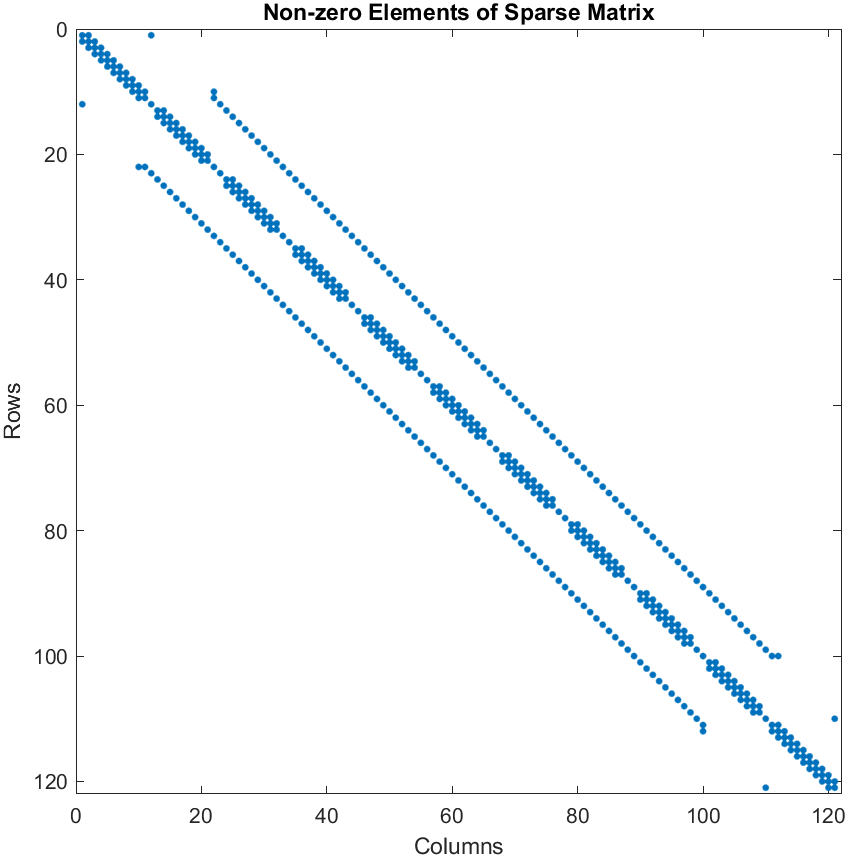
\includegraphics[width=0.5\textwidth]{stiffness.png}
  \caption{Stiffness Matrix}
  \label{fig:stiffness}
\end{figure}

\section{Results}

(1). 求解出满足方程的 $ f(x,y) $
%-((2*cos(x) - (-1+x) .* sin(x)) .* (y-1) .* sin(y) + (x-1) .* sin(x) .* (2*cos(y) - (-1+y).*sin(y)));
\begin{equation}
  \begin{aligned}
    f(x,y) = &((x-1) \cdot \sin(x)-2\cos(x)) \cdot (y-1) \cdot \sin(y)\\
    &((y-1)\cdot\sin(y)-2\cos(y))\cdot(x-1) \cdot \sin(x)
  \end{aligned}
\end{equation}

(2).对区域采用三角形网格剖分 $ \mathcal{T}_h $ ,给出总网格个数、对应的内部结点和边界结点的个数:

使用等距剖分,每个三角形的直角边长为 $ h=1/N$ ,共有 $ 2N^2 $ 个三角形,$ (N+1)^2 $ 个顶点,内部顶点数为 $ (N-1)^2 $ ,边界顶点数为 $ 4N$。

(3). 输出初始网格的结点编号和三角单元的编号方式: 图\ref{fig:triangulation}。

(4). 有限元空间选取分片线性多项式空间。

(5). 输出初始网格对应的刚度矩阵的非零元的图像: 图\ref{fig:stiffness}。

(6). 求解有限元问题,测试程序,并计算 $ L^2,H^1 $ 误差和误差阶。
\begin{table}[htbp]
  \centering
  \begin{tabular}{|c|cc|cc|}
    \toprule
    N & \multicolumn{1}{c}{$L^2$ error} & \multicolumn{1}{c|}{order} & \multicolumn{1}{c}{$H^1$ error} & \multicolumn{1}{c|}{order} \\
    \midrule
    10  & 4.93E-04 &       & 9.27E-03 &       \\
    20  & 1.23E-04 & 1.997 & 4.32E-03 & 1.102 \\
    40  & 3.09E-05 & 1.999 & 2.09E-03 & 1.046 \\
    80  & 7.72E-06 & 2.000 & 1.03E-03 & 1.021 \\  
    \bottomrule
  \end{tabular}%
  \label{tab:error}%
\end{table}%


\end{document}